% Copyright 2007--\today Alexander Grahn
%
% This material is subject to the LaTeX Project Public License. See
%    http://mirrors.ctan.org/help/Catalogue/licenses.lppl.html
% for the details of that license.
%
\documentclass[a4paper]{article}
\frenchspacing
\usepackage[UKenglish]{babel}
\usepackage{xsavebox}
\usepackage{csquotes}
\usepackage{graphicx}
\graphicspath{{files/}}
\usepackage{color}
\usepackage{lmodern}
\usepackage[T1]{fontenc}
\usepackage[protrusion,expansion]{microtype}
\usepackage{parskip}
\usepackage[bookmarksnumbered,linktocpage]{hyperref}
\usepackage{fancyvrb}
\clubpenalty=10000
\widowpenalty=10000
\displaywidowpenalty=10000
\renewcommand{\textfraction}{0.0}
\renewcommand{\topfraction}{1.0}
\renewcommand{\bottomfraction}{1.0}

\hypersetup{
  pdftitle={The xsavebox Package},
  pdfsubject={Documentation},
  pdfauthor={Alexander Grahn},
  pdfkeywords={PDF features, XObject, savebox, LaTeX, dvips, repeated content, repeated graphics, eps, PostScript, ps2pdf, XeLaTeX, pdfLaTeX, LuaLaTeX, dvipdfmx},
  citebordercolor={0 0 1},
  filebordercolor={0 0 1},
  linkbordercolor={0 0 1},
  menubordercolor={0 0 1},
  pagebordercolor={0 0 1},
  urlbordercolor={0 0 1},
%  pdfpagelayout=SinglePage
}

%\usepackage[scaled=0.85]{luximono}

\def\XeLaTeX{X\kern-.1667em\lower.5ex\hbox{\reflectbox{E}}\kern-.125em\LaTeX}
\def\XeTeX{X\kern-.1667em\lower.5ex\hbox{\reflectbox{E}}\kern-.125em\TeX}
\def\pXepLaTeX{(X\kern-.1667em\lower.5ex\hbox{\reflectbox{E}})\kern-.125em\LaTeX}

\def\parsedate#1/#2/#3\relax{
  \def\year{#1}
  \def\month{#2}
  \def\day{#3}
}

\begin{document}
\makeatletter
\title{The {\sffamily xsavebox} Package, v\g@xsb@version@tl}
\expandafter\parsedate\g@xsb@date@tl\relax %set current date to package date
\makeatother
\author{Alexander Grahn\\[1ex]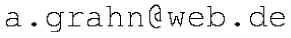
\includegraphics[height=2.7ex]{mailto}}
\maketitle
\begin{abstract}
\noindent This package defines commands for saving content that can be repeatedly placed into the document without replicating DVI/PDF code in the output file, allowing for smaller size of the final PDF file and improved content caching for faster display in certain PDF viewers. The user commands are modelled after the standard \LaTeX{} commands \verb+\savebox+, \verb+\sbox+, \verb+\usebox+ and the `\verb+lrbox+' environment. The package supports all common \TeX{} engines and back-ends, including `\verb+dvips+'.
\end{abstract}

\section{Introduction}
Whenever the standard \LaTeX{} command \verb+\usebox{+\emph{save-box}\verb+}+ is issued to insert a previously defined \emph{save-box} more than once, the typeset content stored therein is written as DVI or PDF code into the output file again. The redundant code adds to the overall file size and may impair the page caching facilities built into some PDF viewers.

The PDF file format defines a powerful mechanism for packing readily typeset content once into self-contained entities, so-called \enquote{Form XObjects}, that can be referenced at other places within the PDF document.

The `\verb+xsavebox+' package makes this PDF feature accessible on the \LaTeX{} level as a set of user commands which look similar to and are used in a similar way as the well-known \emph{save-box} related \LaTeX{} commands.

All common \TeX{} engines and back-ends are supported, which are:
\begin{itemize}
%\item $\varepsilon$-\TeX
\item pdf\LaTeX, Lua\LaTeX,
\item \LaTeX{} $\rightarrow$ \verb+dvips+ $\rightarrow$ \verb+ps2pdf+/Distiller
\item \pXepLaTeX{} $\rightarrow$ \verb+(x)dvipdfmx+
\end{itemize}

To enable `\verb+dvipdfmx+', pass it as a document class option.

It should be emphasized that \enquote{Form XObjects} is a PDF feature. Content saved and referenced using \enquote{Form XObjects} is only visible in the final PDF output, but not in intermediate formats of the work-flow if those are involved, namely DVI and PostScript. Of course, PostScript converted back from PDF displays the content correctly.

\section{Package Options}
\begin{Verbatim}
margin=<dimension>  
\end{Verbatim}
When content is converted into a Form XObject, it is clipped to its bounding box. However, the glyphs of the fonts which are used for typesetting tend to be slightly bigger than their boxes. In order to avoid clipping, the `\verb+xsavebox+' package \emph{temporarily} adds an additional margin of \verb+3pt+ around the content. In rare cases, \verb+3pt+ may turn out to be insufficient, e.\,g. if text is up-scaled before being put into a save box. This option allows the setting of a larger margin to ensure that the content gets entirely into the save box. Note that whichever value is chosen for `\verb+margin+', the spacing of the boxes, when inserted into the document, remains unchanged. This is what every user definitely wants.

\section{User commands}
\subsection*{Content saving}
\vspace{-1\baselineskip}
\hrulefill\\[-1.6\baselineskip]
\begin{Verbatim}
\xsbox{<xsbox name>}{<content>}
\xsavebox{<xsbox name>}[<width>][<position>]{<content>}
\xsavebox*{<xsbox name>}[<width>][<position>]{<content>}

\begin{xlrbox}{<xsbox name>}
  <content>
\end{xlrbox}

\begin{xlrbox*}{<xsbox name>}
  <content>
\end{xlrbox*}
\end{Verbatim}
\vspace{-1\baselineskip}
\hrulefill\\[-1\baselineskip]

The main difference of these commands as compared to their standard \LaTeX{} counterparts without the leading `\verb+x+' is the way of naming boxes. The label \verb+<xsbox name>+ is an identifier that may be composed of arbitrary non-active characters, including spaces and numbers. A command for declaring a box register \verb+<xsbox name>+ does not exist.

The \verb+[<width>]+ and \verb+[<position>]+ options have the same meaning as with \verb+\savebox+ and \verb+\makebox+. As usual, the additional length commands
\begin{Verbatim}
  \width
  \height
  \depth
  \totalheight
\end{Verbatim}
are defined for use in the \verb+[<width>]+ option and refer to the original dimensions of \verb+<content>+. The value of \verb+<position>+ may assume one of `\verb+l+', `\verb+r+', `\verb+c+' or `\verb+s+'. The default is `\verb+c+' for text centred in the box.

\verb+<content>+ is typeset in LR-mode. Longer text to be typeset in paragraph mode must be put into a \verb+\parbox+ or `\verb+minipage+'.

The starred (`\verb+*+') versions of the commands allow for later colour injection into the boxes at the place of their referencing. The colour which is active at the time of building the box is not saved with the content. This feature only works with pdf\LaTeX{} and Lua\LaTeX.

Note that
\begin{Verbatim}
  \xsbox{image for frequent use}{\includegraphics{example}}  
\end{Verbatim}
is useful only in the \LaTeX{} $\rightarrow$ \verb+dvips+ $\rightarrow$ \verb+ps2pdf+ work-flow, as all other engines and back-ends already take care of preventing multiple graphics file inclusion.

Verbatim content can only be saved using the `\verb+xlrbox[*]+' environment.

With \LaTeX{} in DVI mode and \XeLaTeX, box \emph{saving} commands should not be placed on a line of their own with empty lines above and below. For technical reasons this will produce an empty paragraph. Always place them at the beginning or at the end of a paragraph in the input file. Also, box saving commands cannot be placed in the document preamble with \LaTeX{} (DVI) and \XeLaTeX{}.

\subsection*{Referencing saved content}
Previously saved content can be inserted with\\[-1.6\baselineskip]

\hrulefill\\[-1.6\baselineskip]
\begin{Verbatim}
\xusebox{<xsbox name>}
\end{Verbatim}
\vspace{-1ex}
or
\vspace{-1ex}
\begin{Verbatim}
\the<xsbox name>
\end{Verbatim}
\vspace{-1\baselineskip}
\hrulefill\\[-1\baselineskip]

The second, shorthand form can be used if \verb+<xsbox name>+ is composed exclusively of letters (`\verb+a+`--`\verb+z+', `\verb+A+`--`\verb+Z+'). For example, a box named `\verb+MyFirstExample+' could be referenced as
\begin{Verbatim}
  \theMyFirstExample
\end{Verbatim}
but a box named `\verb+My 1st Example ;-)+' would require
\begin{Verbatim}
  \xusebox{My 1st Example ;-)}
\end{Verbatim}

The referencing commands \verb+\xusebox{<xsbox name>}+ and \verb+\the<xsbox name>+ can again be placed inside the \verb+<content>+ body of box saving commands. There is no upper limit of nesting levels.

\verb+\xusebox{<xsbox name>}+ and \verb+\the<xsbox name>+ behave exacly like common \TeX{} boxes. Therefore, they can be scaled, rotated and resized using the corresponding commands from the `\verb+graphicx+' package.

\section{Example}
An example with colour injection (pdf\LaTeX/Lua\LaTeX-only) follows:

\begin{xlrbox*}{SavedPar}
  \begin{minipage}[b]{1in}
  silly boxed paragraph that no one will ever use
  \end{minipage}
\end{xlrbox*}%
Here is a \fbox{\color{blue}\theSavedPar} for anything.

The same \fbox{\color{green}\rotatebox{90}{\theSavedPar}} was inserted again but with a different colour and rotated by 90 degree.

\begin{Verbatim}
\usepackage{xsavebox}  
\usepackage{color}
\usepackage{graphicx}
...
\begin{xlrbox*}{SavedPar}% `*' --> no colour at the time of saving
  \begin{minipage}[b]{1in}
  silly boxed paragraph that no one will ever use
  \end{minipage}
\end{xlrbox*}
%colours injected into \theSavedPar
Here is a \fbox{\color{blue}\theSavedPar} for anything.

The same \fbox{\color{green}\rotatebox{90}{\theSavedPar}} was
inserted again but with a different colour and rotated by 90 degree.
\end{Verbatim}

\end{document}
